\documentclass{article}

% 导入中文宏包
\usepackage{ctex}
\usepackage{array}
\usepackage{caption}
\usepackage{hyperref}
% 设置页面边距
\usepackage{geometry}
\usepackage{graphicx}
\geometry{a4paper, left=2.5cm, right=2.5cm, top=3cm, bottom=3cm}

% 设置标题、作者和日期
\title{实验报告二:Vim和Shell工具脚本的学习}
\author{23020007011崔涛}

\begin{document}

% 生成标题、作者和日期
\maketitle

% 心得报告正文
\section{实验目的}
学习使用Vim编辑器和Shell工具和脚本,熟悉一些基本操作,方便以后的学习和工作需要。

\section{介绍}
\subsection{Vim和Shell简介}
Vim是一个强大的文本编辑器,从vi发展而来,被程序员广泛使用。它不仅支持代码补全、编译及错误跳转等功能,还通过语法高亮等方式方便编程

Shell是Linux系统中与操作系统内核交互的接口,充当命令解释器的角色。最常用的shell环境是bash。Shell脚本能够批量执行一系列命令,非常适用于自动化任务

Vim和Shell在Linux使用中各有其独特之处,它们提供了从文本编辑到系统管理、自动化任务处理的全面功能。掌握它们对于每个Linux用户来说都是必要的,不仅能提高工作效率,还能深入理解Linux系统的运作方式。
\section{练习内容}
\subsection{Vim学习样例}
1.在默认设置下,Vim 会在左下角显示当前的模式。Vim 启动时的默认模式是正常模式。

可以按下 \verb|<ESC>|(退出键)从任何其他模式返回正常模式。在正常模式,键入 \verb|i| 进入插入 模式,\verb|R| 进入替换模式,\verb|v| 进入可视(一般)模式,\verb|V| 进入可视(行)模式,\verb|<C-v>| (Ctr进入可视(块)模式,\verb|:| 进入命令模式。

 

2. \verb|vim +/关键字 文件路径可以高亮显示关键字,如图1所示
\begin{figure}
    \centering % 使图片居中
    \includegraphics[width=\textwidth]{"vim1.png"}
    \caption{这是第二个例子的图片。} % 图片的标题
    \label{fig:example} % 为图片设置标签,以便引用
\end{figure}

3.在正常模式下键入 \verb|:| 进入命令行模式。 在键入 \verb|:| 后,你的光标会立即跳到屏幕下方的命令行。 这个模式有很多功能,包括打开,保存,关闭文件,以及 退出 Vim 
    
\begin{itemize}
    \item \verb|:q| 退出(关闭窗口)
    \item \verb|:w| 保存(写)
    \item \verb|:wq| 保存然后退出
    \item \verb|:e {文件名}| 打开要编辑的文件
    \item \verb|:ls| 显示打开的缓存
    \item \verb|:help {标题}| 打开帮助文档
        \item \verb|:help :w| 打开 \verb|:w| 命令的帮助文档
        \item \verb|:help w| 打开 \verb|w| 移动的帮助文档
\end{itemize}

   
4.
    
\begin{itemize}
    \item \verb|d{移动命令}| 删除 \{移动命令\}
例如,\verb|dw| 删除词, \verb|d$| 删除到行尾, \verb|d0| 删除到行头。

    \item \verb|c{移动命令}| 改变 \{移动命令\}
    \begin{itemize}
        \item 例如,\verb|cw| 改变词
        \item 比如 \verb|d{移动命令}| 再 \verb|i|
    \end{itemize}
    \item \verb|x| 删除字符(等同于 \verb|dl|)
    \item \verb|s| 替换字符(等同于 \verb|xi|)
    \item 可视化模式 + 操作
选中文字, \verb|d| 删除 或者 \verb|c| 改变

    \item \verb|u| 撤销, \verb|<C-r>| 重做
    \item \verb|y| 复制 / “yank” (其他一些命令比如 \verb|d| 也会复制)
    \item \verb|p| 粘贴
    \item  \verb|~| 改变字符的大小写
\end{itemize}
 
 

5\verb|   :s| (替换)命令。

\begin{itemize}
    \item \verb|%s/foo/bar/g|
在整个文件中将 foo 全局替换成 bar

    \item \verb|%s/\[.*\](\(.*\))/\1/g|
将有命名的 Markdown 链接替换成简单 URLs

\end{itemize}
 

6.
Vim 命令 / 宏

\begin{itemize}
    \item \verb|ggdd|, \verb|Gdd| 删除第一行和最后一行
    \item 格式化最后一个元素的宏 (寄存器 \verb|e|)
    \begin{itemize}
        \item 跳转到有 \verb|<name>| 的行
        \item \verb|qe^r"f>s": "<ESC>f<C"<ESC>q|
    \end{itemize}
    \item 格式化一个 的宏
    \begin{itemize}
        \item 跳转到有 \verb|<person>| 的行
        \item \verb|qpS{<ESC>j@eA,<ESC>j@ejS},<ESC>q|
    \end{itemize}
    \item 格式化一个 标签然后转到另外一个 的宏
    \begin{itemize}
        \item 跳转到有 \verb|<person>| 的行
        \item \verb|qq@pjq|
    \end{itemize}
    \item 执行宏到文件尾
\verb|999@q|

    \item 手动移除最后的 \verb|,| 然后加上 \verb|[| 和 \verb|]| 分隔符
\end{itemize}

7.
安装和配置插件 \verb|ctrlp.vim| 


\begin{itemize}
    \item 用 \verb|mkdir -p ~/.vim/pack/vendor/start| 创建插件文件夹
    \item 下载这个插件: \verb|cd ~/.vim/pack/vendor/start; git clone https://github.com/ctrlpvim/ctrlp.vim|

下载后需要在\~/.vimrc 中添加如下设置,

\begin{verbatim}
 \textbf{set} runtimepath^=~/.vim/pack/vendor/start/ctrlp.\textbf{vim} 
\end{verbatim}

\end{itemize}
 
8.
安装 vim-plug 
\begin{itemize}
\item 输入这串指令\newline curl -fLo ~/.vim/autoload/plug.vim --create-dirs \
https://raw.githubusercontent.com/junegunn/vim-plug/master/plug.vim
\item 修改 ~/.vimrc\newline call plug#begin()\newline
 Plug 'preservim/NERDTree' #需要安装的插件 NERDTree\newline
 Plug 'wikitopian/hardmode'  #安装 hardmode\newline
 call plug#end()
 \item 在 vim 命令行中执行 \verb|:PlugInstall| 
\end{itemize}

9.
打开vim内置的教程,输入命令vimtutor。跟随教程可以得到一些基本的vim指导。 



10.
输入vimdiff  加上两个文件名即可轻松实现两个文档的对比!


\subsection{Shell学习样例10个}
1.阅读 \verb|man ls| ,然后使用 \verb|ls| 命令进行如下操作:

\begin{itemize}
    \item 所有文件(包括隐藏文件)
    \item 文件打印以人类可以理解的格式输出 (例如,使用 454M 而不是 454279954)
    \item 文件以最近访问顺序排序
    \item 以彩色文本显示输出结果
\end{itemize}
 

\noindent
\begin{minipage}{\linewidth}
  \centering
  % 插入图片
  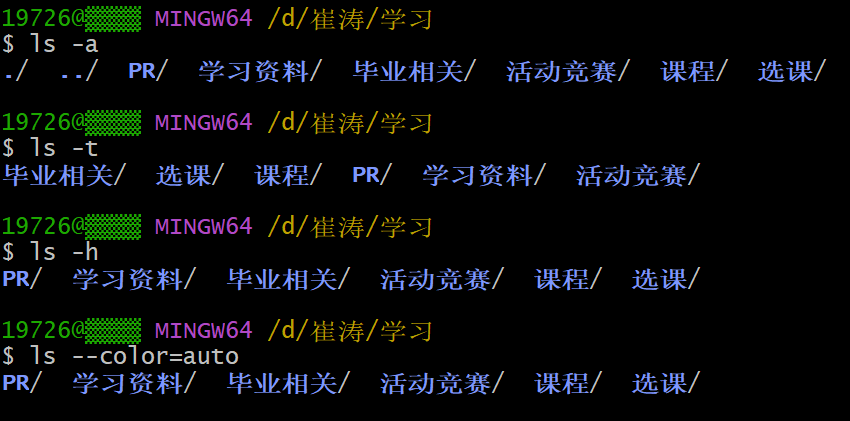
\includegraphics[width=0.5\linewidth]{Shell1.png}
  % 图片标题
  \captionof{figure}{ls指令查看文件}
  \label{fig:example}
\end{minipage}


2.
编写两个 bash 函数 \verb|marco| 和 \verb|polo| 执行下面的操作。 每当你执行 \verb|marco| 时,当前的工作目录应当以某种形式保存,当执行 \verb|polo| 时,无论现在处在什么目录下,都应当 \verb|cd| 回到当时执行 \verb|marco| 的目录。
\newline
解答:新建一个.sh文件,向文件中写入如下函数,然后执行source指令,随后再运行marco和polo即可\newline。#!/bin/bash\newline
 marco(){\newline
     echo "$(pwd)" > $HOME/marco_history.log\newline
     echo "save pwd $(pwd)"
 }\newline
 polo(){\newline
     cd "$(cat "$HOME/marco_history.log")"\newline
 }\newline
 
 


\noindent
\begin{minipage}{\linewidth}
  \centering
  % 插入图片
  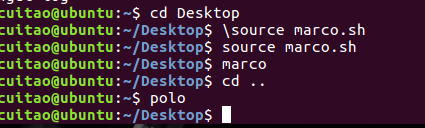
\includegraphics[width=0.5\linewidth]{Shell2.png}
  % 图片标题
  \captionof{figure}{编写简单脚本}
  \label{fig:example}
\end{minipage}

3.假设您有一个命令,它很少出错。因此为了在出错时能够对其进行调试,需要花费大量的时间重现错误并捕获输出。 编写一段 bash 脚本,运行如下的脚本直到它出错,将它的标准输出和标准错误流记录到文件,并在最后输出所有内容。 加分项:报告脚本在失败前共运行了多少次。 
\newline
解答:
 编写如下bash测试脚本,然后执行source指令,随后再运行即可。\newline
 \newline\newline\newline
 if [[ n -eq 42 ]]; then\newline
     echo "Something went wrong"\newline
     >\&2 echo "The error was using magic numbers"\newline
     exit 1\newline
 fi\newline

 echo "Everything went according to plan"\newline
~                                           

\noindent
\begin{minipage}{\linewidth}
  \centering
  % 插入图片
  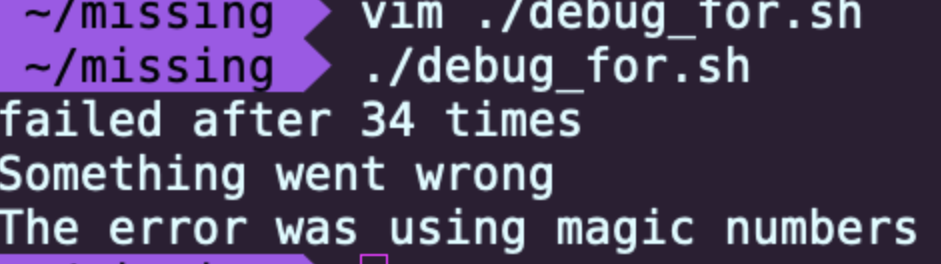
\includegraphics[width=0.5\linewidth]{Shell3.png}
  % 图片标题
  \captionof{figure}{测试脚本的编写}
  \label{fig:example}
\end{minipage}

4.编写一个命令,它可以递归地查找文件夹中所有的 HTML 文件,并将它们压缩成 zip 文件。注意,即使文件名中包含空格,您的命令也应该能够正确执行 \newline

首先创建所需的文件 \newline
\begin{verbatim}
 mkdir html_root 
 cd html_root
 touch \textbf{{}1..10\textbf{}}.html
 mkdir html
 cd html 
 touch xxxx.html
\end{verbatim}
 \newline
 随后执行如下的find指令查看所有HTML文件并将其压缩为ZIP文件。\newline
 find . -type f -name "*.html" | xargs -d 'n'  tar -cvzf html.zip\newline
 

\noindent
\begin{minipage}{\linewidth}
 \centering
  % 插入图片
  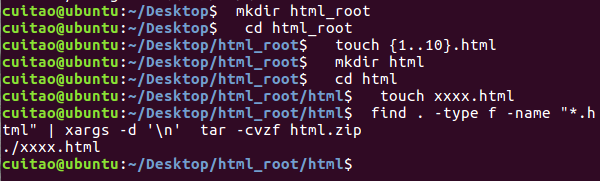
\includegraphics[width=0.5\linewidth]{Shell4.png}
  % 图片标题
  \captionof{figure}{查看指定格式并压缩文件}
  \label{fig:example}
\end{minipage}

5.
编写一个命令或脚本递归的查找文件夹中最近使用的文件 \newline
解答:输入以下命令即可\newline find . -type f -print0 | xargs -0 ls -lt | head -1\newline
\noindent
\begin{minipage}{\linewidth}
 \centering
  % 插入图片
  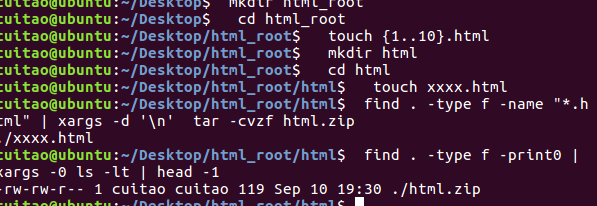
\includegraphics[width=0.5\linewidth]{Shell5.png}
  % 图片标题
  \captionof{figure}{查找最近使用文件}
  \label{fig:example}
\end{minipage}

6.当执行脚本时,我们经常需要提供形式类似的参数。bash 使我们可以轻松的实现这一操作,它可以基于文件扩展名展开表达式。这一技术被称为 shell 的 \textit{通配}
\begin{itemize}
    \item 通配符 当想要利用通配符进行匹配时,你可以分别使用 \verb|?| 和 \verb|*| 来匹配一个或任意个字符。例如,对于文件 \verb|foo|, \verb|foo1|, \verb|foo2|, \verb|foo10| 和 \verb|bar|, \verb|rm foo?| 这条命令会删除 \verb|foo1| 和 \verb|foo2| ,而 \verb|rm foo*| 则会删除除了 \verb|bar| 之外的所有文件。
    \item 花括号 \verb|{}| - 当有一系列的指令,其中包含一段公共子串时,可以用花括号来自动展开这些命令。这在批量移动或转换文件时非常方便。
\end{itemize}
 

\noindent
\begin{minipage}{\linewidth}
 \centering
  % 插入图片
  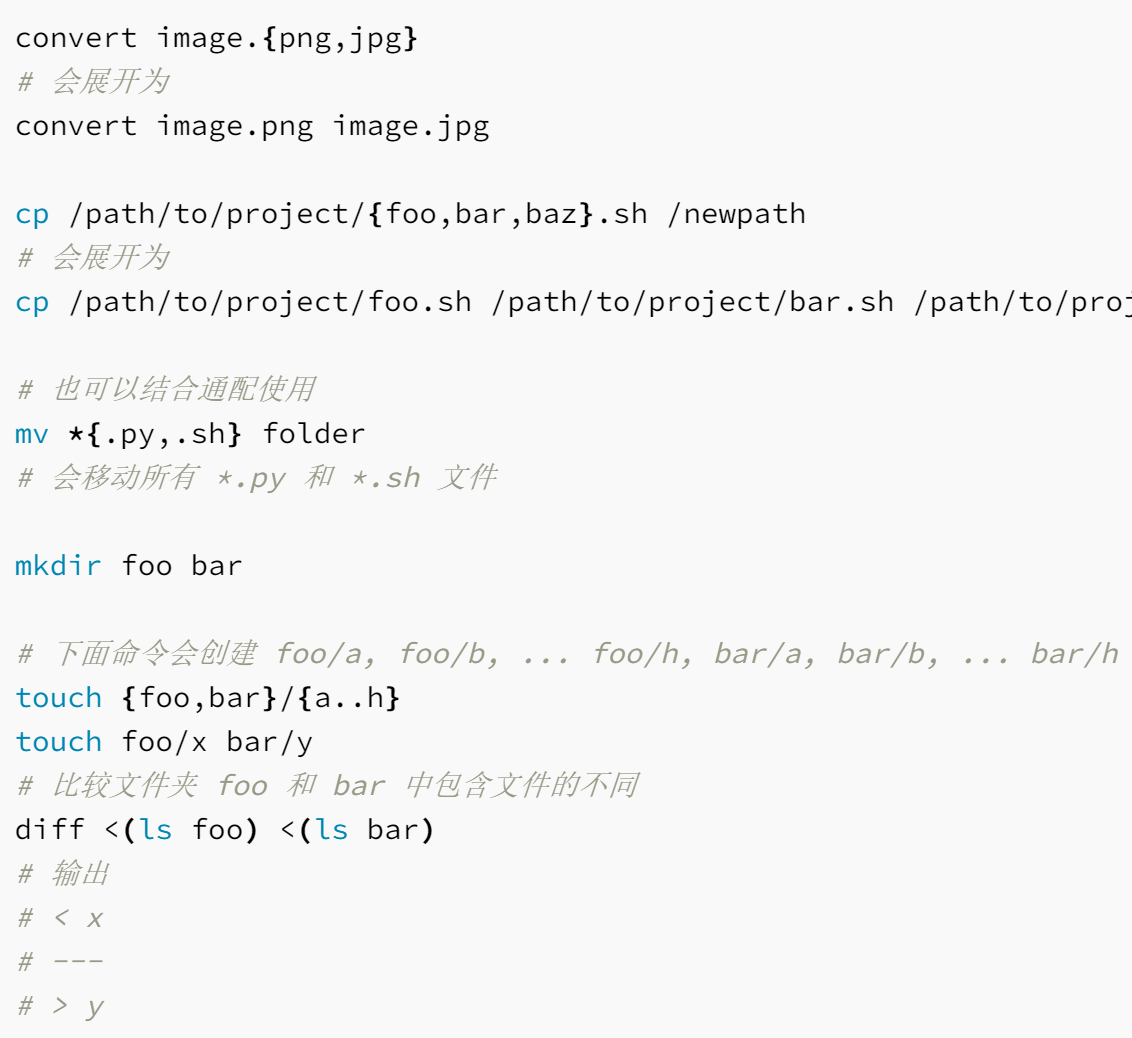
\includegraphics[width=0.5\linewidth]{Shell6.png}
  % 图片标题
  \captionof{figure}{Shell命令中通配符的使用}
  \label{fig:example}
\end{minipage}

7.所有的类 UNIX 系统都包含一个名为 \href{https://man7.org/linux/man-pages/man1/find.1.html}{\verb|find|} 的工具,它是 shell 上用于查找文件的绝佳工具。\verb|find| 命令会递归地搜索符合条件的文件,例如查找前一天修改过的文件。

\noindent
\begin{minipage}{\linewidth}
 \centering
  % 插入图片
  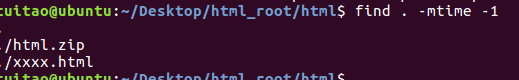
\includegraphics[width=0.5\linewidth]{Shell7.png}
  % 图片标题
  \captionof{figure}{利用find来查找前一天修改的文件}
  \label{fig:example}
\end{minipage}

8.\verb|history| 命令允许您以程序员的方式来访问 shell 中输入的历史命令。这个命令会在标准输出中打印 shell 中的历史命令。如果我们要搜索历史记录,则可以利用管道将输出结果传递给 \verb|grep| 进行模式搜索。 \verb|history | grep find| 会打印包含 find 子串的命令。 

\noindent
\begin{minipage}{\linewidth}
 \centering
  % 插入图片
  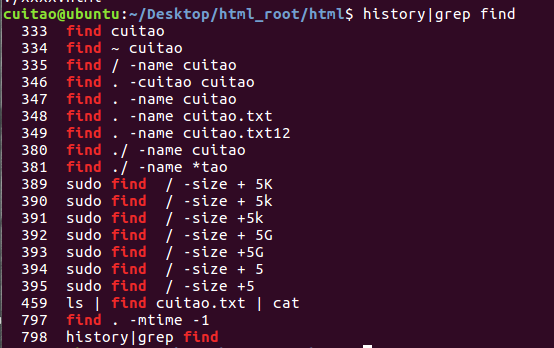
\includegraphics[width=0.5\linewidth]{Shell8.png}
  % 图片标题
  \captionof{figure}{查找以往命令记录}
  \label{fig:example}
\end{minipage}

9.alias 是 Bash 内建命令,用来设置命令的别名。 
\newline
alias [-p] [NAME[=VALUE] ...] \newline

10.
\subparagraph{chmod 命令}

\begin{itemize}
    \item \verb|ls -lh| 显示当前目录所有文件的权限
    \item \verb|chmod 777 |文件名 修改文件权限(最高权限)
\end{itemize}
\section{解题感悟}
在初步接触Vim和Shell后,我不禁对这两个工具的强大功能和灵活性感到惊讶。作为计算机科学的初学者,我原以为图形界面的编辑器和操作系统是现代编程的标配。然而,通过学习Vim和Shell,我发现命令行界面同样能够提供高效、直观的操作环境。\newline
在学习Vim的过程中,最初我对它的模式切换感到困惑,为何一个简单的文本编辑器需要如此复杂的操作模式?但当我逐渐习惯了这种模式之后,我意识到这是Vim设计哲学的一部分,旨在提高编辑效率。我可以不用离开键盘就能完成大部分文本编辑任务,这显著加快了我的工作速度。使用hjkl键进行移动,以及各种快捷命令,如dd和yy,让我感受到了Vim的威力。更不用说,Vim脚本和插件的可扩展性为我定制自己的工作环境提供了无限可能。\newline
转向Shell的学习,我开始了解到命令行。Shell不仅仅是一个简单的命令执行器,它是一种强大的脚本语言,允许我自动化日常任务、处理文件和数据流、甚至编写复杂的程序。学习如何使用管道、重定向、和正则表达式,让我能够以前所未有的方式处理文本数据。此外,Shell脚本让我能够将常用的命令序列保存为脚本,实现一键执行,极大提升了我的工作效率。
总的来说,虽然Vim和Shell的学习对我比较困难,但一旦掌握,它们就会成为了我的工具箱中不可或缺的工具。它们不仅提高了我的编程效率,还让我对计算机的工作方式有了更深入的理解。我期待着继续探索它们的高级功能,并将这些知识应用到更广泛的计算机科学领域中去。

github路径
您可以在此查看我的源代码: 

\url{https://github.com/cuitao223/myhomework}
\end{document}
